\documentclass[12pt, a4paper]{article}
\usepackage[utf8]{inputenc}
\usepackage[IL2]{fontenc}
\usepackage[czech]{babel}
\usepackage{graphicx}

\begin{document}


\begin{figure}[h!]
\centering

\includegraphics[width=75mm]{favlogo.jpg}
\end{figure}

{\centering
{\huge Internet Control Message Protocol}\\[1em]
{\large ICMPv4}\\[1em]
{\large KIV/PSI - semestrální práce}\\[11,5cm]
}

\begin{tabular}{l r}
student: & Radek VAIS\\
os. číslo: & A17N0093P\\
mail: & vaisr@students.zcu.cz\\
datum: & 10.6.2018\\
\end{tabular}

\thispagestyle{empty}
\newpage

%========================================
%========================================
%========================================
%========================================
%========================================
\section{Zadání} %=====================================================================================================

Úloha bude mít dvě části. Část analytickou a část syntetickou. V~analytické části budete analyzovat pakety nebo rámce vybraného protokolu. Jako zdroj poslouží nějaký standardní program. V~Syntetické části vygenerujete vlastní pakety nebo rámce, odešlete je ověřenému (standardnímu) protějšku, který vygeneruje odpověď. Jak Vaši výzvu, tak i odpověď zachytíte prvním programem a zobrazíte. Pochopitelně první i druhá část může tvořit jeden celek.

Předkládané programové vybavení musí obsahovat i část ladicí, která nebude samoúčelná, ale bude sloužit k~odladění programu i k~odladění výměny zpráv. Ladicí výpis by měl obsahovat zejména časový údaj, dále pak informaci o~úrovni ladění a vlastní ladicí text. Můžete se inspirovat Syslogem.

Programová a uživatelská dokumentace bude součástí komprimovaného balíčku, který odevzdáte. Balíček bude kromě toho také obsahovat zdrojové kódy v~samostatných adresářích a makefile pro Linux. Dokumentace v~tištěné podobě se neodevzdává. Semestrální práce se odevzdávají na Courseware.

Zvoleným protokolem je ICMP - Internet Control Message protocol ve verzi 4.
%========================================
\newpage

\section{Analýza}

Dle RFC-792 Protokol ICMPv4 slouží k~technické kontrole sítě a úpravě toku dat a reportování chyb. K~přenosu zpráv mezi uzly je použit protokol IP, z~toho důvodu ICMP nemůže detekovat chyby IP protokolu. Typickou situací generování ICMP zprávy je nedoručitelný datagram z~důvodů malé vyrovnávací paměti uzlu na cestě. Nejedná se o~spolehlivý protokol, ani není jeho cílem udělat IP protokol spolehlivým. Hlavním důvodem vzniku protokolu bylo předávání zpětné vazby o~problémech v~komunikaci. Na ICMP zprávy se nelze spolehnout při implementaci spolehlivosti vyšší vrstvy ze dvou důvodů. Prvním je, že v~případě chyby ICMP zpráva nemusí být vygenerována. Druhým je fakt, že při chybě přenosu ICMP zprávy se negeneruje nová ICMP zpráva. Takové chování by způsobovalo zahlcení "poškozené" sítě.

IP záhlaví zprávy ICMP protokolu vypadá následujícím způsobem:

\begin{verbatim}
 0                   1                   2                   3
 0 1 2 3 4 5 6 7 8 9 0 1 2 3 4 5 6 7 8 9 0 1 2 3 4 5 6 7 8 9 0 1
+-+-+-+-+-+-+-+-+-+-+-+-+-+-+-+-+-+-+-+-+-+-+-+-+-+-+-+-+-+-+-+-+
|Ver = 4|  IHL  |Ty. of Ser. =0 |          Total Length         |
+-+-+-+-+-+-+-+-+-+-+-+-+-+-+-+-+-+-+-+-+-+-+-+-+-+-+-+-+-+-+-+-+
|         Identification        |Flags|      Fragment Offset    |
+-+-+-+-+-+-+-+-+-+-+-+-+-+-+-+-+-+-+-+-+-+-+-+-+-+-+-+-+-+-+-+-+
|  Time to Live |  Protocol = 1 |         Header Checksum       |
+-+-+-+-+-+-+-+-+-+-+-+-+-+-+-+-+-+-+-+-+-+-+-+-+-+-+-+-+-+-+-+-+
|                       Source Address                          |
+-+-+-+-+-+-+-+-+-+-+-+-+-+-+-+-+-+-+-+-+-+-+-+-+-+-+-+-+-+-+-+-+
|                    Destination Address                        |
+-+-+-+-+-+-+-+-+-+-+-+-+-+-+-+-+-+-+-+-+-+-+-+-+-+-+-+-+-+-+-+-+
|                    Data....                                  
+-+-+-+-+-+-+-+-+-+-+-+-

\end{verbatim}

Jednotlivá pole IP záhlaví jsou definovány následujícím způsobem:

\begin{itemize}
\item Ver = version = verze IP protokolu - hodnota 4 pro IPv4.
\item IHL = internet header lenght = velikost IP záhlaví.
\item Ty. of Ser. = Type of service = nároky na zpracování zprávy - hodnota 0 pro ICMP zprávy.
\item Total Length = délka celé zprávy.
\item Identification, Flags, Fragment Offset - pole pro informace o~fragmentaci zprávy.
\item Time to Live = doba života zprávy.
\item Protocol = Protokol nesený IP zprávou - hodnota 1 pro ICMP.
\item Checksum = kontrolní součet - doplněk součtu 16 bitových slov.
\item Source Address = zdrojové adresa IPv4.
\item Destination Address = cílová adresa IPv4.
\item Data = prostor pro data nesená ICMP protokolem.
\end{itemize}

Záhlaví ICMP zprávy je dlouhé 8 bytů, většina zpráv využívá pouze první 4byty, které jsou definované následujícím způsobem:

\begin{verbatim}
 0                   1                   2                   3
 0 1 2 3 4 5 6 7 8 9 0 1 2 3 4 5 6 7 8 9 0 1 2 3 4 5 6 7 8 9 0 1
+-+-+-+-+-+-+-+-+-+-+-+-+-+-+-+-+-+-+-+-+-+-+-+-+-+-+-+-+-+-+-+-+
| Type          | Code          | Checksum                      |
+-+-+-+-+-+-+-+-+-+-+-+-+-+-+-+-+-+-+-+-+-+-+-+-+-+-+-+-+-+-+-+-+
\end{verbatim} 

Jednotlivá pole ICMP záhlaví jsou definovány následujícím způsobem:

\begin{itemize}
\item Type = Typ zprávy ICMP.
\item Code = Přesnější zařazení ICMP zprávy.
\item Checksum = Doplněk součtu 16 bitových slov celé ICMP zprávy.
\end{itemize}

\subsection{Typy zpráv}

Přehled ICMP zpráv:

\begin{enumerate}
\item Echo Reply (Type = 0)
\item Destination Unreachable (3)
\item Source Quench (4)
\item Redirect (5)
\item Echo (8)
\item Time Exceeded (11)
\item Parameter Problem (12)
\item Timestamp (13)
\item Timestamp Reply (14)
\item Information Request (15)
\item Information Reply (16)
\end{enumerate}

\subsubsection{Destination unreachable}

Pokud nebyl nalezený záznam o~žádané sítí, protokolu, zařízení nebo portu je odeslána zpráva "Destination unreachable". Pole Code obsahuje identifikaci, jaký element nebyl nalezen. Dále je v~datech ICMP zprávy uložena hlavička původního IP packetu a 64 bitů dat. 

\subsubsection{Time Exceeded}

Pokud packetu vypršela doba života, uzel je povinen ho zahodit. A~může notifikovat zdroj zprávou "Time Exceeded", která v~datech obsahuje IP záhlaví originální zprávy + 64 bitů dat. Pokud k~vypršení času došlo v~důsledku čekání na jednotlivé fragmenty zprávy, bude pole Code nastaveno na hodnotu 1.

\subsubsection{Parameter problem}

Pokud uzel při přijetí IP packetu zjistí, že některá z~hodnot IP záhlaví je chybná odešle zprávu "Parameter problem". V~datech této zprávy bude uvedeno IP záhlaví originální zprávy + 64 bitů dat. Dále tento typ zprávy využívá další byte záhlaví, pro označení ve kterém bytu záhlaví zprávy došlo k~chybě.

\subsubsection{Source quenche}

V~případě, že uzel zahodil zprávu z~důvodů malého bufferu pro zpracování, může notifikovat zdroj zprávou "Source quenche". V~datech této zprávy bude uvedeno IP záhlaví originální zprávy + 64 bitů dat.

\subsubsection{Redirect}

Zpráva slouží k~upravení směrování na lokálním segmentu. V~případě, že je do hraničního směrovače oblasti odeslána zpráva, kterou směrovač odešle jinému směrovači ve stejné síti, zároveň odešle zprávu "Redirect". V~dalších 4bytech záhlaví je uložena IPv4 adresa nové brány a data obsahují originální IP záhlaví + 64 bitů dat. 

\subsubsection{Echo a Echo Reply}

Zpráva slouží k~ověření, zda cílový uzel je v~provozu. Tato ICMP zpráva využívá všch 8bytů záhlaví. První dva doplňující byty obsahují identifikační hodnotu zprávy druhé dva pak sekvenční číslo jednotlivých zpráv. Dotazovaný uzel je povinen odeslat zpět celou část uvedenou v~poli data zpět zdrojovému uzlu.

\subsubsection{Timestamp a Timestamp Reply Message}

Zpráva slouží ke zjištění odhadu časového průchodu zprávy sítí. Stejně jako zpráva Echo využívá zpráva Timestamp celé záhlaví ICMP se shodným významem identifikace a sekvenčního čísla. V~datech pak využívá 3x32 bitů pro uložení časů odeslání, přijetí na vzdáleném uzlu a odeslání na vzdáleném uzlu. Čas je uložen ve formátu počet \emph{ms} od půlnoci času UTC.

\subsubsection{Information Request a Information Reply Message}

Zprávy slouží ke zjištění adresy sítě, kde je host připojen. Je možné odeslat zprávu s~nevyplněnou cílovou IP adresou. Opět je využito celé ICMP záhlaví ve smyslu identifikace a sekvenčního čísla (viz Echo). Data nejsou odesílána.

\subsection{Zranitelnosti}

Základní zranitelností ICMP protokolu je nízká úroveň filtrace ICMP zpráv. Protože korektní fungování ICMP protokolu na síti je prospěšné správnému fungování, nejsou ICMP zprávy filtrovány firewally. Lze tak použít ICMP zprávu ECHO k~přenosu dat na jiný kompromitovaný uzel. Protože je ICMP neautorizovaný, je často využíván k~DoS útokům. 
Nejznámější DoS útok pomosí ICMP zpráv je Smurf attack (Šmoulí útok). Při Smurf útoku útočník odesílá packety ICMP ECHO, které mají jako zdrojovou adresu uvedenou broadcastovou adresu cílové stanice. Útočník očekává, že napadená stanice vygeneruje ICMP ECHO REPLY s~B/C adresou svého segmentu a zahltí je tak svým provozem.
Dalším DoS útokem s~pomocí ICMP je Black Nurse. Tento útok slouží k~zahlcení firewallů pomocí generování zpráv ICMP DESTINATION UNREACHBLE (port unreachable). Útočník očekává, že se firewally zahltí pří zpracovávání informací o~nedostupnosti.

\section{Implementace protokolu}

V~rámci praktické části semestránlí práce vznikl program, který přijímá a zobrazuje příchozí ICMP zprávy. Dále je možné pomocí tohoto programu generovat zprávy Echo, Timestamp a Information request.  

\subsection{Návrh aplikace}

Aplikace se skládá ze dvou modulů \texttt{icmp} a \texttt{gui}. Modul \texttt{icmp} obsahuje definice, logiku přijímání a odesíání zpráv. Modul \texttt{gui} obsahuje uživatelské rozhraní.

\subsubsection{Modul ICMP}

Základem modulu ICMP je definice struktury ICMP záhlaví a následně objektu \texttt{ICMPMessage}, který poskytuje metody, pro nastavení parametrů záhlaví a uložení dat zprávy. Poslední funkcionalitou tohoto objektu je serializace nastavených dat do pole unifikovaných bytů (\texttt{uint8\_t}).

Asynchronní příjem a odesílání zpráv je zaručen paralelním během dvou vláken (jedno pro odesílání, druhé pro příjem). Každé vlákno před před spuštěním vytvoří instanci ICMP socketu pomocí volání \emph{socket()}. Vlákno odesílání pracuje nad frontou zpráv dle návrhového vzoru producent konzument. Vlákno příjmu, neprodleně propisuje prijaté ICMP zprávy do GUI prostřednictvím rozhraní definovaném třídou \texttt{GUIInterface}. Celý proces běhu vláken je spravován pomocí řídící třídy \texttt{Messenger}. Tato třída obsahuje vlajky pro běch jednotlivých vláken unikátní instanci fronty odesílaných zpráv.

Fornta odesílaných zpráv je instance objektu \texttt{MessageQueue}. Tento objekt je implementace blokující fronty. Pro synchronizaci jsou využity prostředky systémové knihoveny C++ \texttt{<mutex>}, pro uložení dat je využita knihovna \texttt{<list>}.

\subsubsection{Modul GUI}

K~implementaci uživatelského rozhraní byly použity prostředky knihovny \emph{Qt} verze 5. Uživatelské rozhraní obsahuje dvě okna. Pro strukturální popis oken je použito XML pro definici UI ve frameworku \emph{Qt}\footnote{Definice Qt UI XML - http://doc.qt.io/archives/qt-4.8/designer-ui-file-format.html}. Modul \texttt{gui} dále obsahuje definici datového modelu pro zobrazované zprávy a definici objetů zobrazovaných zpráv. Posledním elementem tohoto modulu je definice rozhraní \texttt{GUIInterface}, které slouží ke komunikaci obou modulů.

\subsection{Překlad}

Cílovou platformou programu je \emph{OS GNU/Linux}, z~důvodů závisloti na implementaci knihoven pro práci se sockety (\texttt{<sys/socket.h>}). Další závislostí je přítomnost frameworku Qt na sestavovací stanici.

K~překladu je nutné využít mechanismů frameworku \emph{Qt}. Nejprve je potřeba spustit program \texttt{qmake} ve složce s~projektovým souborem \texttt{ICMPSniffer.pro}. Výstupem tohoto programu je soubor \emph{Makefile}, který dodržuje závilosti modulů a respektuje nastavení stanice, na které byl spuštěn. Druhým krokem pro sestavení programu je spuštění \texttt{make} nad vygenerovaným \emph{Makefile}. Výstupem tohoto volání je spustitelný program.

\subsection{Ovládání}

Pro běh programu je nutné mít nainstalovanou knihovnu \emph{Qt} ve verzi 5 a vyšší. Program lze spustit z~grafického rozhraní i z~konzole. V~případě spuštění z~konzole bude mít uživatel k~dispozici log událostí aplikace.

\begin{figure}[h!]
\centering
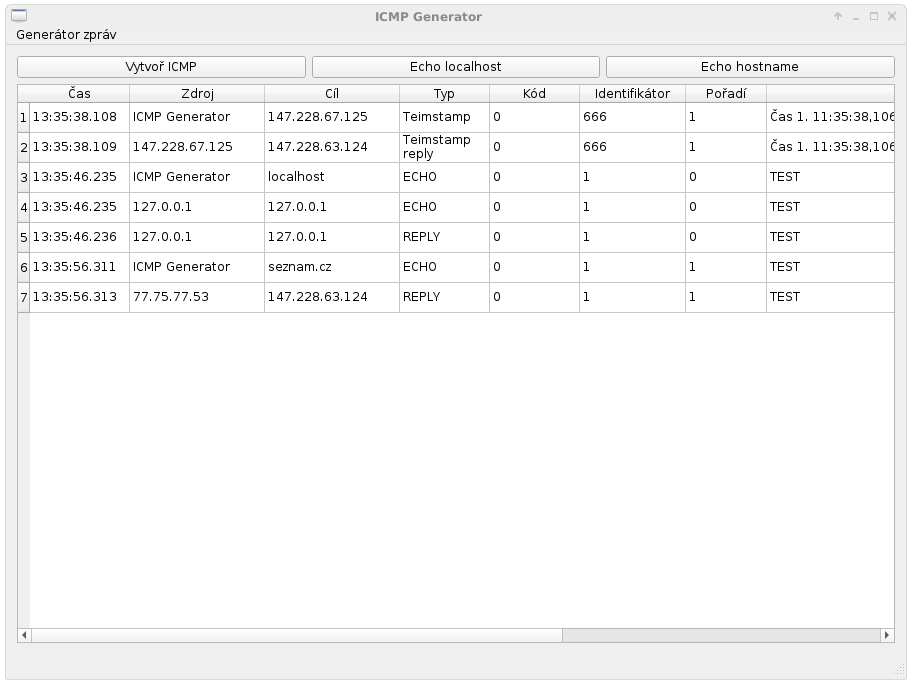
\includegraphics[width=110mm]{gui.png}
\caption{Uživatelské rozhraní aplikace.}
\label{gui}
\end{figure}

Spuštění programu může selhat v~případě, že se nepovede otevřít ICMP socket. Návratový kód programu je \texttt{1} v~příadě, že se nepodařilo otevřít socket pro odesílání zpráv a \texttt{3} v~případě, že se nepodařilo otevřít a správně nastavit IP socket pro přijímání zpráv.

Po spuštění uživatelského rozhraní se zobrazí okno viz Obrazáek \ref{gui}. Uživatel má k~dispozici tři akce. První je odeslat zprávu ECHO s~předdefinovaným textem "TEST" na adresu localhost. Druhou je odeslání zprávy ECHO s~předdefinovaným textem na adresu dle určení. Poslední možností je vytvořit vlastní ICMP zprávu.

Možnost vytvoření ICMP zprávy poskytuje uživateli možnost generovat tři typy zpráv: Echo, Timestamp a Information request. Uživatel má plnou kontrolu nad vyplněním parametrů jednotlivých zpráv.

\begin{figure}[h!]
\centering
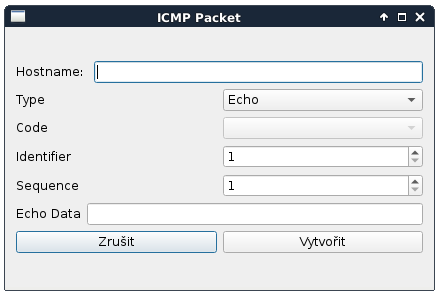
\includegraphics[width=110mm]{gui2.png}
\label{gui2}
\caption{Rozhraní pro generování packetů.}
\end{figure}


\newpage

\section{Závěr}

V~rámci této práce byl vytvořen program pro příjímání, zobrazování a syntézu ICMP zpráv. Pro zobrazovnání zpráv bylo vytvořeno uživatelské rozhraní ve framworku \emph{Qt}.

Během testování aplikace byla ověřena funkčnost syntétzy a příjmu zpráv ECHO proti standardní implementaci protokolu (např. zařízení na adrese seznam.cz). Pouze v~laboratoři byla oveřena funkčnost zpráv Timestamp, proti standardní implementaci ICMP ve Windows 10 stanic v~laboratoři. Zpráva Information request byla pouze zachycena a prozkoumána programem \emph{Wireshark}, bohužel standardní Information response se nepodařilo zachytit.

\end{document}